\chapter{Amélioration de la Modélisation des Intersections et Changements de Voie}
\label{chap:intersections}

Ce chapitre présente une modélisation détaillée des intersections et des changements de voie dans le contexte spécifique du trafic béninois, en mettant l'accent sur le comportement particulier des motos à ces points critiques du réseau.

\section{Conditions aux Limites Dynamiques}
\label{sec:conditions_limites}

Les intersections constituent des points singuliers dans le réseau routier, où les conditions de continuité du flux sont modifiées par les entrées et sorties de véhicules.

\subsection{Formulation Mathématique pour les Intersections}
\label{subsec:formulation_intersections}

Pour une intersection située en $x = x_0$, nous définissons les conditions aux limites suivantes :

\begin{empheq}[box=\colorbox{lightblue!15}]{align}
\lim_{x \to x_0^-} \sum_{i=1}^N \flowi{i}(x,t) = \lim_{x \to x_0^+} \sum_{i=1}^N \flowi{i}(x,t) + \Delta q(t)
\label{eq:condition_limite}
\end{empheq}

où $\Delta q(t)$ représente la variation nette du flux à l'intersection (positive pour une entrée nette, négative pour une sortie nette).

Pour chaque classe de véhicule $i$, nous avons également :

\begin{align}
\lim_{x \to x_0^+} \flowi{i}(x,t) = \alpha_i(t) \cdot \lim_{x \to x_0^-} \sum_{j=1}^N \flowi{j}(x,t) + \beta_i(t)
\label{eq:flux_classe_intersection}
\end{align}

où :
\begin{itemize}
\item $\alpha_i(t)$ est la proportion du flux entrant attribuée à la classe $i$;
\item $\beta_i(t)$ est le flux additionnel spécifique à la classe $i$ (par exemple, flux de motos entrant par un accès informel).
\end{itemize}

\subsection{Traitement des Feux de Circulation}
\label{subsec:feux_circulation}

Pour les intersections régulées par des feux de circulation, $\Delta q(t)$ devient une fonction périodique dépendant du cycle des feux :

\begin{align}
\Delta q(t) = 
\begin{cases}
g(t) \cdot q_{\max} & \text{pendant le feu vert} \\
0 & \text{pendant le feu rouge}
\end{cases}
\label{eq:delta_q_feux_detaille}
\end{align}

La fonction $g(t)$ module l'efficacité du flux pendant la phase verte et intègre plusieurs phénomènes observés dans le contexte béninois :

\begin{align}
g(t) = g_0 \cdot (1 - e^{-(t-t_s)/\tau_1}) \cdot (1 - (1-\gamma) \cdot (1 - e^{-(t_e-t)/\tau_2}))
\label{eq:fonction_g}
\end{align}

où :
\begin{itemize}
\item $g_0$ est l'efficacité maximale de l'intersection;
\item $t_s$ est l'instant de début du feu vert;
\item $t_e$ est l'instant de fin du feu vert;
\item $\tau_1$ est le temps caractéristique d'accélération au démarrage;
\item $\tau_2$ est le temps caractéristique de décélération à l'approche du feu rouge;
\item $\gamma$ est le facteur de non-respect du feu rouge (particulièrement pertinent pour les motos).
\end{itemize}

\begin{figure}[htbp]
\centering
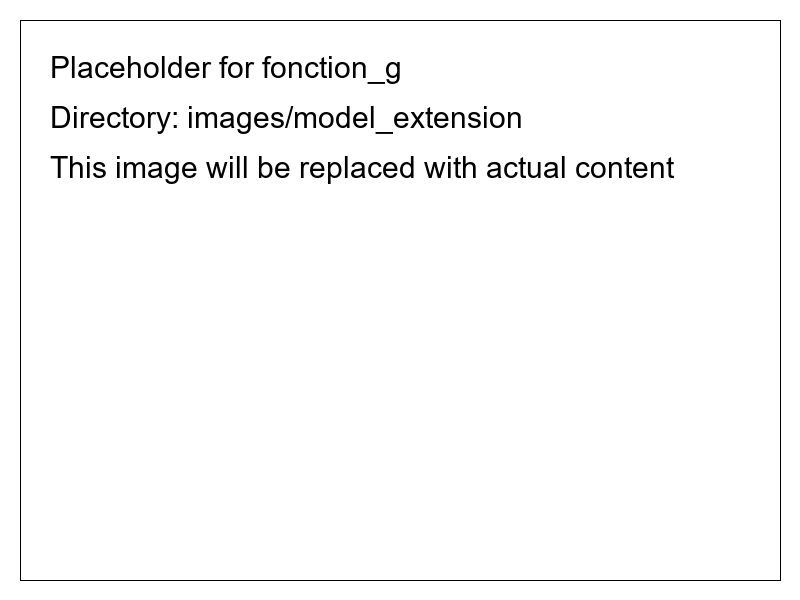
\includegraphics[width=0.8\textwidth]{images/model_extension/fonction_g}
\caption{Fonction de modulation $g(t)$ pour différentes classes de véhicules : (a) forme générale sur un cycle complet; (b) zoom sur la phase de démarrage; (c) zoom sur la phase d'arrêt.}
\label{fig:fonction_g}
\end{figure}

Les paramètres $\tau_1$, $\tau_2$ et $\gamma$ diffèrent significativement entre les classes de véhicules, reflétant notamment la plus grande agilité des motos et leur tendance à anticiper le feu vert et à ignorer le feu rouge:

\begin{table}[htbp]
\centering
\caption{Paramètres de la fonction $g(t)$ par classe de véhicule}
\label{tab:parametres_g}
\begin{tabular}{lccc}
\toprule
\textbf{Classe de véhicule} & $\tau_1$ (s) & $\tau_2$ (s) & $\gamma$ \\
\midrule
Motos & 2.1 & 3.5 & 0.35 \\
Voitures particulières & 4.5 & 5.2 & 0.05 \\
Taxis & 3.8 & 4.9 & 0.12 \\
Bus & 6.2 & 8.3 & 0.02 \\
Camions & 7.5 & 9.1 & 0.01 \\
\bottomrule
\end{tabular}
\end{table}

\subsection{Adaptation aux Intersections Non Régulées}
\label{subsec:intersections_non_regulees}

Pour les intersections sans feux de circulation (majoritaires au Bénin), nous utilisons un modèle basé sur la priorité et les gaps critiques :

\begin{align}
\Delta q(t) = \sum_{i=1}^N q_{i,\text{in}}(t) \cdot P_i(t) - \sum_{i=1}^N q_{i,\text{out}}(t)
\label{eq:flux_non_regule}
\end{align}

où $P_i(t)$ est la probabilité qu'un véhicule de classe $i$ puisse s'insérer dans le flux principal, déterminée par :

\begin{align}
P_i(t) = \exp\left(-\lambda_{\text{conf}} \cdot \sum_{j=1}^N \flowi{j}(t) \cdot (t_{g,i} - t_{m,j}) \right)
\label{eq:probabilite_insertion}
\end{align}

avec :
\begin{itemize}
\item $\lambda_{\text{conf}}$ : intensité du conflit à l'intersection;
\item $t_{g,i}$ : gap critique pour la classe $i$;
\item $t_{m,j}$ : temps moyen entre deux véhicules de classe $j$ dans le flux principal.
\end{itemize}

Pour les motos, le gap critique $t_{g,M}$ est significativement plus petit que pour les autres véhicules, reflétant leur capacité à s'insérer dans des espaces réduits.

\section{Interactions Locales}
\label{sec:interactions_locales}

Les interactions entre véhicules aux intersections et lors des changements de voie sont particulièrement importantes dans le contexte béninois, où le comportement des motos modifie significativement la dynamique du trafic.

\subsection{Modélisation des Conflits}
\label{subsec:conflits}

Nous modélisons les conflits entre différentes classes de véhicules à l'aide d'une matrice d'interaction $\boldsymbol{\Gamma} = [\gamma_{ij}]$, où $\gamma_{ij}$ quantifie l'impact d'un véhicule de classe $j$ sur un véhicule de classe $i$.
